% !TEX root = ../my_thesis.tex

\section{Training des Convolutional Neural Networks}
cnns werden erst modelliert und anschließend traniert.
posenet caffe implementierung
Trainingsdaten sind die synthetischen Daten und Testdaten sind die realen Daten

\subsection{Erhebung der echten Daten}
Es wurden für die Aufgabenstellung interessante Aufnahmezonen in der Gebäudesimulation festgelegt und anschließend die Aufnahmen durchgeführt. Für die Aufnahmen wurden zeitgleich zwei unterschiedliche Kameras der Intel Realsense Reihe verwenden. Eine Intel Realsense T265\footnote{\url{https://www.intelrealsense.com/tracking-camera-t265/} (abgerufen am: 18.07.2019)}, die über Inertial Measurement Units (\textit{IMU}) und zwei Fischaugenkameras die Odometrie ermittelt, wurde eingesetzt. Zudem wurde eine Intel Realsense D435\footnote{ \url{https://www.intelrealsense.com/depth-camera-d435/} (abgerufen am: 18.07.2019)}, die eine 3D Punktwolke, ein Tiefenbild sowie ein RGB-Bild einer Szene liefert, benutzt. Die T265 wurde über die D435 Kamera montiert, siehe Abbildung .... Über das Robot Operating System\footnote{\url{https://www.ros.org/about-ros/} (abgerufen am: 18.07.2019)} (\textit{ROS}) Framework wurden die Kameras zeitgleich angesprochen und der Datenfluss diverser Sensoren synchronisiert. Somit beinhaltet jeder Datensatz zwei Bildern der Fischaugenkameras, ein Tiefenbild, ein RGB-Bild, eine 3D Punktwolke und die dazugehörige Odometrie pro Szene (Vgl. Abbildung 1). Für diese Arbeit sind nur die Odometrie-Daten der T265 sowie die RGB-Bilder der D435 relevant.



\begin{figure}[h!]
	\centering
	\begin{subfigure}[b]{0.3\linewidth}
		\centering
		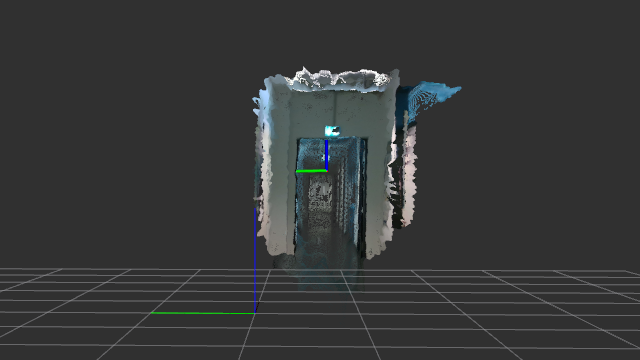
\includegraphics[width=\linewidth]{images/dataset/pointcloud3.png}
		\caption{Odometrie  (\textit{T265}) + \\ Punktwolke (\textit{D435})}
	\end{subfigure}
	\hfill
	\begin{subfigure}[b]{0.3\linewidth}
		\centering
		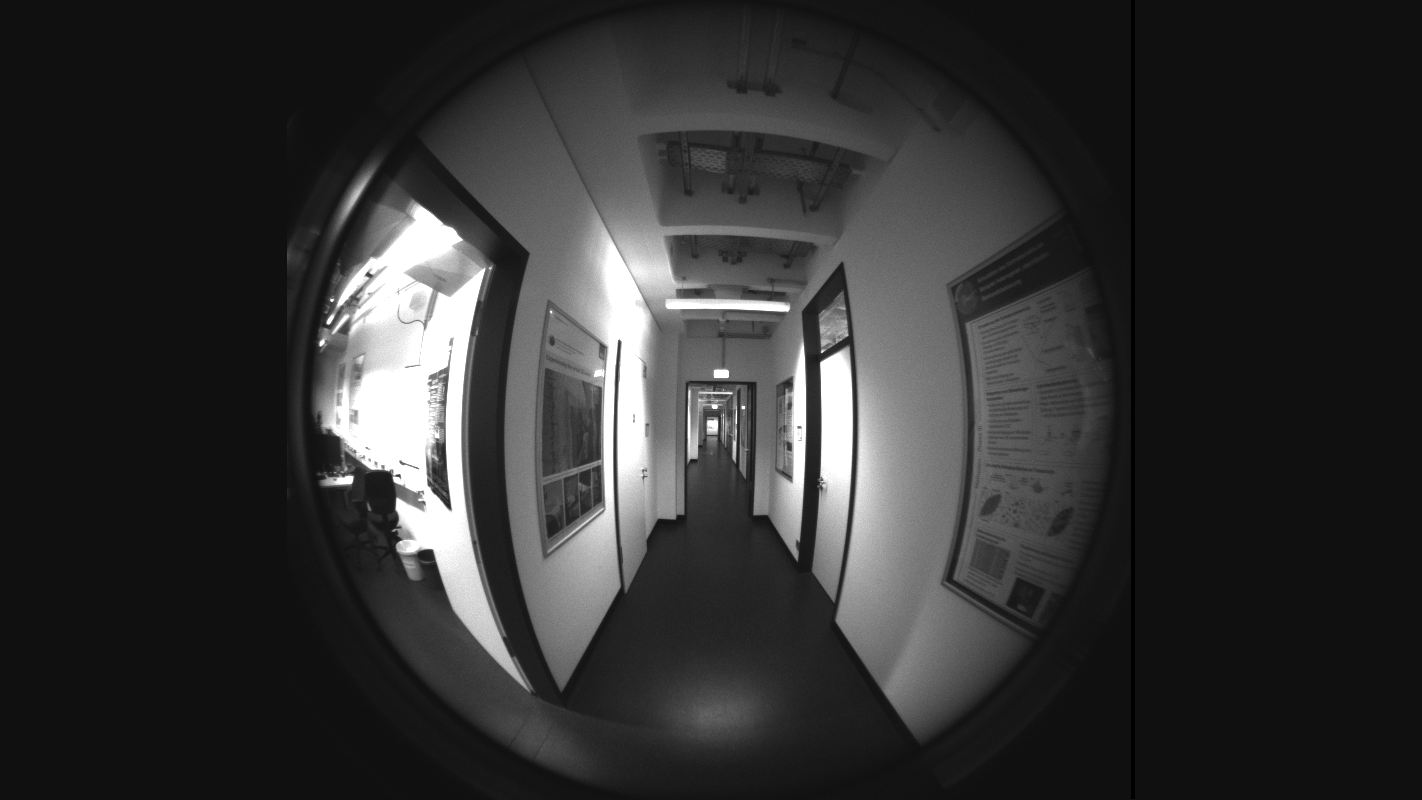
\includegraphics[width=\linewidth]{images/dataset/f1_frame000005.png}
		\caption{Fischaugenkamera 1 \\ (\textit{T265})}
	\end{subfigure}
	\hfill
	\begin{subfigure}[b]{0.3\linewidth}
		\centering
		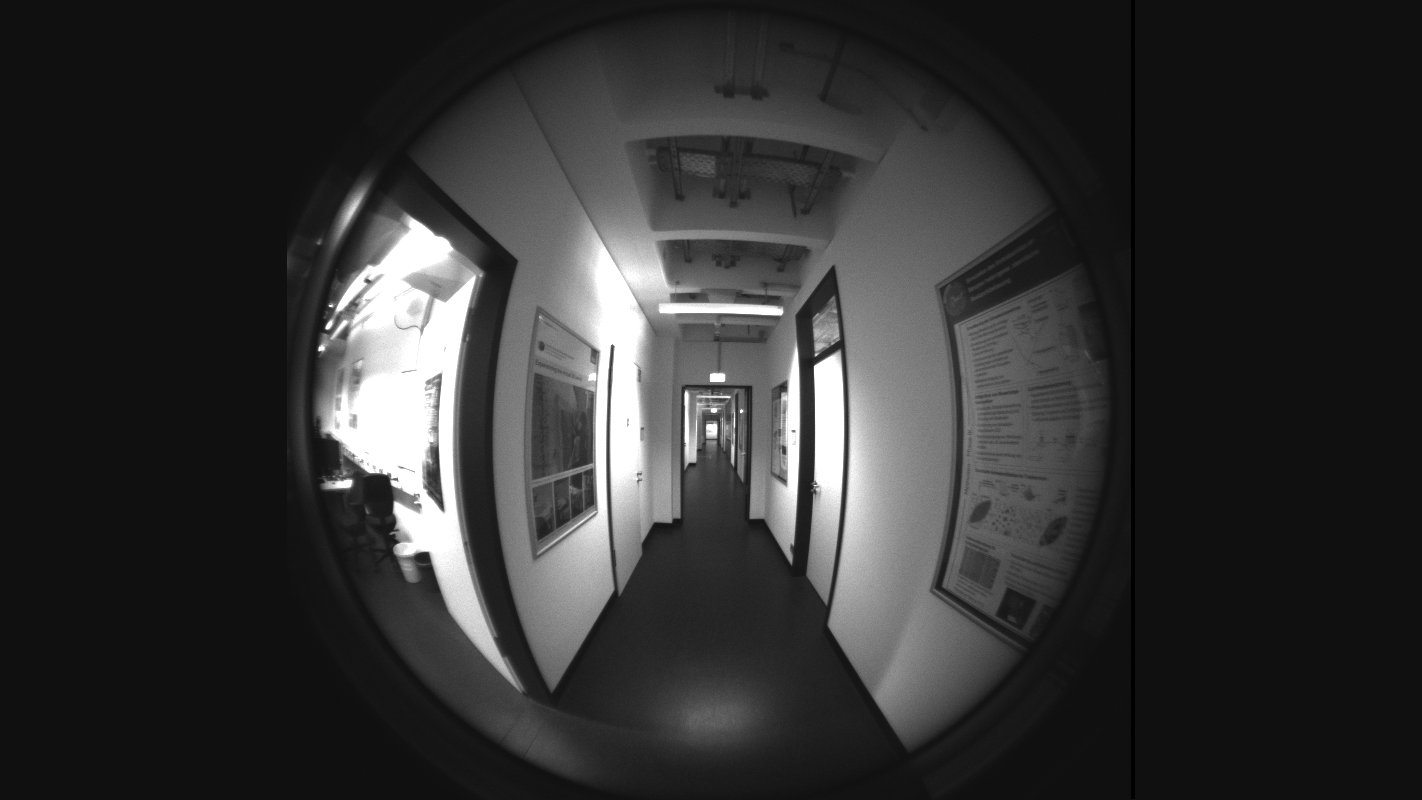
\includegraphics[width=\linewidth]{images/dataset/f2_frame000005.png}
		\caption{Fischaugenkamera 2 \\ (\textit{T265})}
	\end{subfigure}
	\medskip
	\begin{subfigure}[b]{0.3\linewidth}
		\centering
	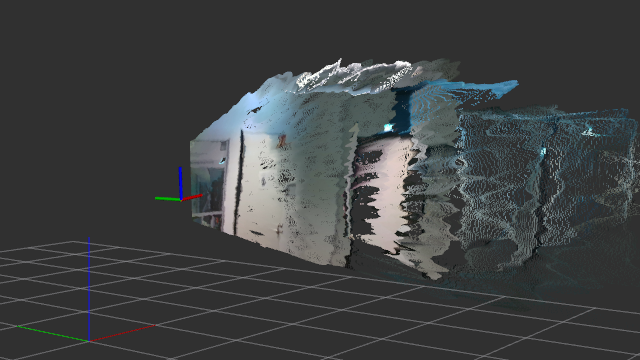
\includegraphics[width=\linewidth]{images/dataset/pointcloud1.png}
	\caption{Odometrie  (\textit{T265}) + \\ Punktwolke (\textit{D435})}
	\end{subfigure}
	\hfill
	\begin{subfigure}[b]{0.3\linewidth}
		\centering
		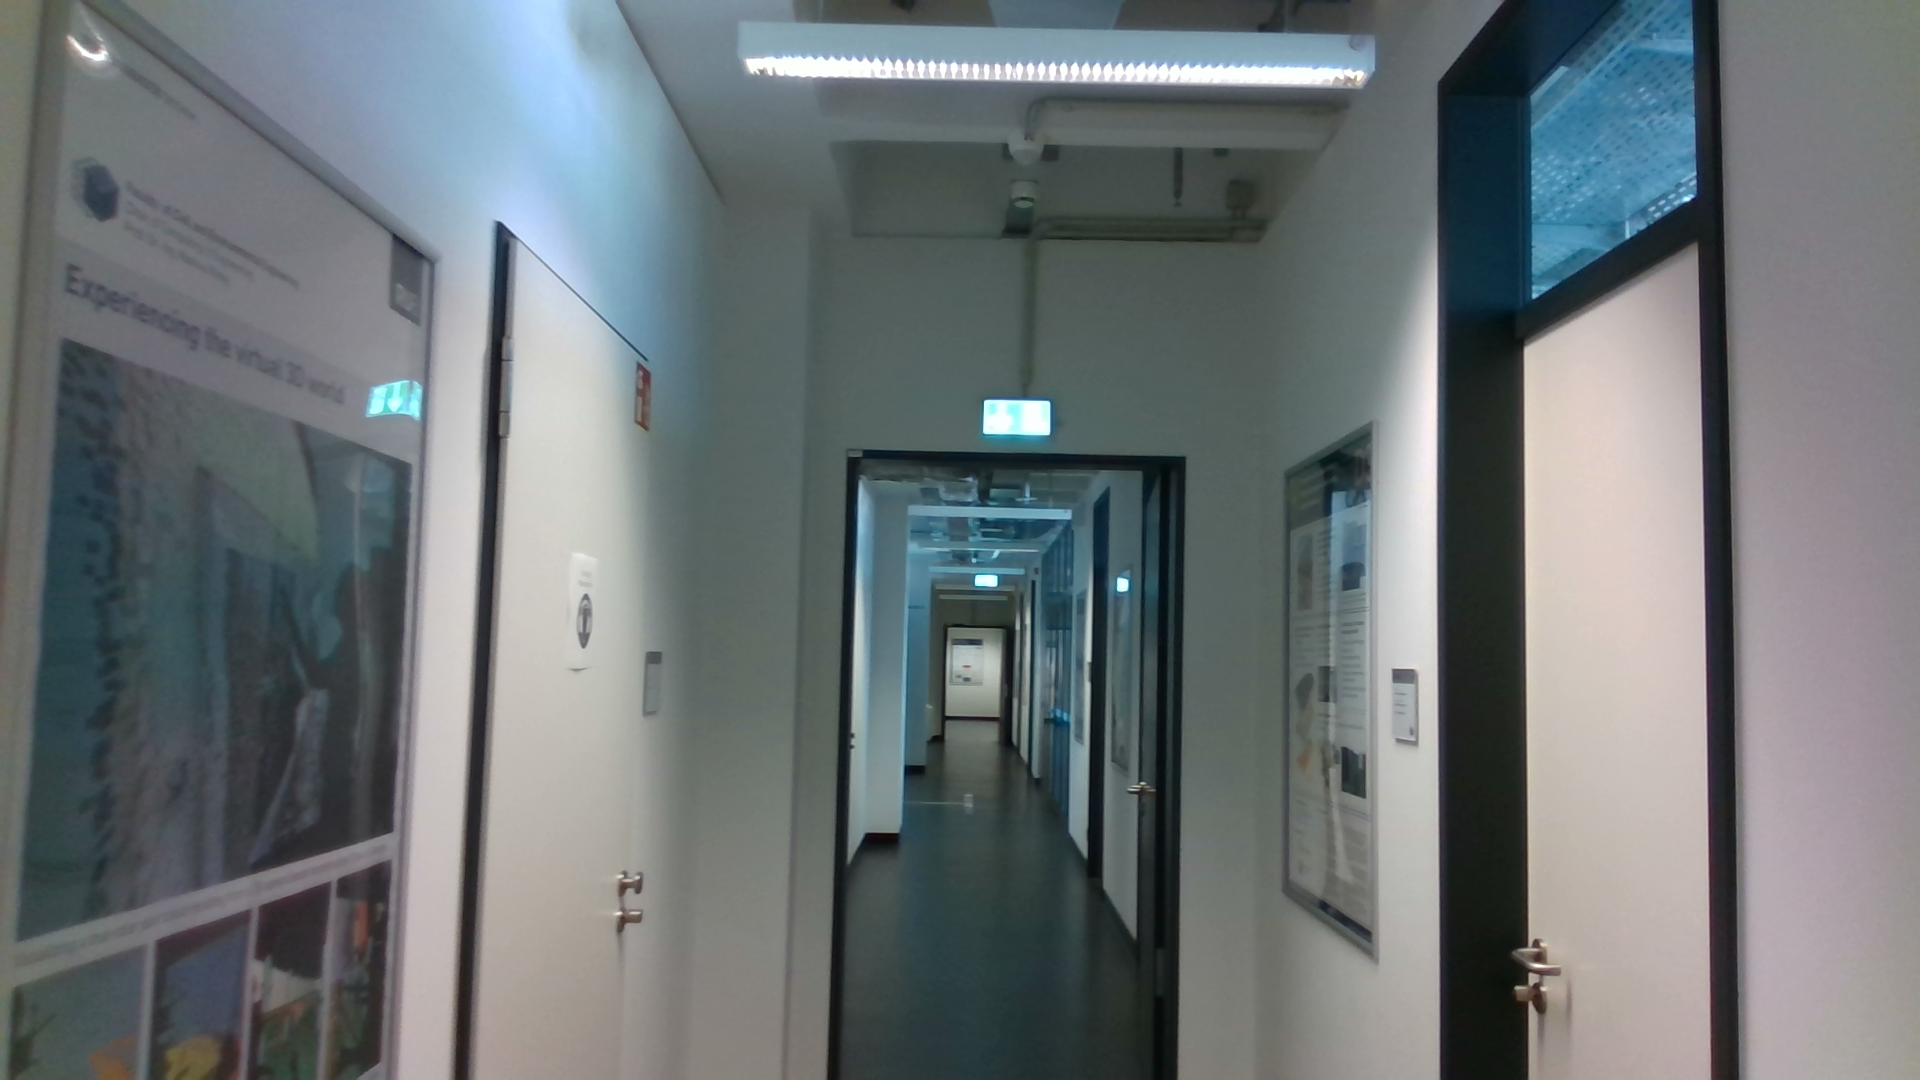
\includegraphics[width=\linewidth]{images/dataset/dc_frame000005.png}
		\caption{RGB-Bild \\ (\textit{D435}) \hspace*{2cm}}
	\end{subfigure}
	\hfill
	\begin{subfigure}[b]{0.3\linewidth}
		\centering
		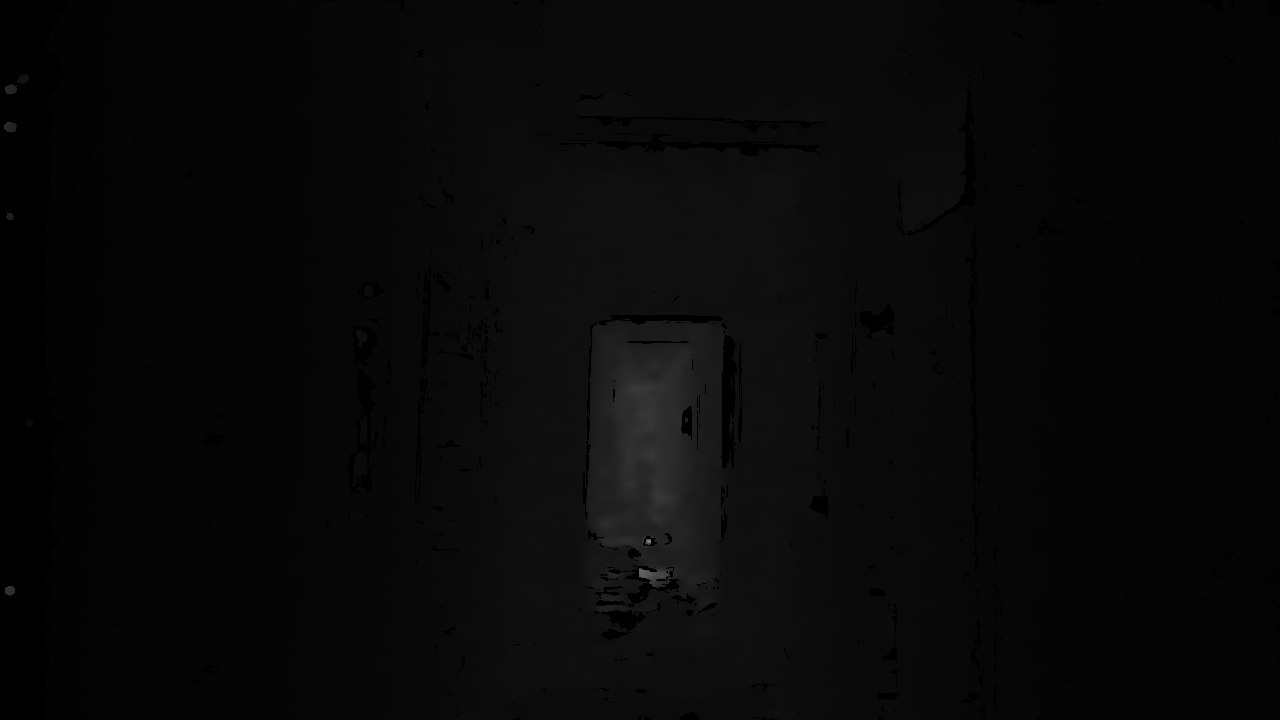
\includegraphics[width=\linewidth]{images/dataset/dt_frame000005.png}
		\caption{Tiefenbild \\ (\textit{D435}) \hspace*{2cm}}
	\end{subfigure}
	\caption{The same cup of coffee. Multiple times.}
	\label{fig:coffee3}
\end{figure}


\subsection{Generierung der synthetischen Daten}
Blender,
eigenes Addons erstellt ein Kamerakonstrukt, das ein NURBs-Pfad entlag aufnimmt; Variation der Orientierung; ...

\subsection{Verarbeitung der Daten}
// gradienten\\
Bei der Erzeugung von Gradienten- bzw. Kantenbilder gehen einerseits wichtige Informationen im Hinblick auf das Ursprungsbild verloren, andererseits bleiben wichtige Informationen wie z.B. die geometrische Struktur erhalten.

\subsection{Trainingsparameter}
optimizer, beta,
learningrate,
weights decay, anz. data; ...